\documentclass[12pt,a4paper]{article}

\usepackage[utf8]{inputenc}
\usepackage[T1]{fontenc}
\usepackage{lmodern}
\usepackage{microtype}
\usepackage{geometry}
\usepackage{amsmath,amssymb,amsfonts}
\usepackage{booktabs}
\usepackage{array}
\usepackage{graphicx}
\usepackage{float}
\usepackage{caption}
\usepackage{subcaption}
\usepackage{enumitem}
\usepackage{xcolor}
\usepackage{hyperref}
\usepackage[numbers,sort&compress]{natbib}

\geometry{margin=2.45cm}
\hypersetup{
  colorlinks=true,
  linkcolor=blue!55!black,
  citecolor=blue!55!black,
  urlcolor=blue!55!black
}
\graphicspath{{figures/}}
\setlist[itemize]{topsep=3pt,itemsep=2pt,parsep=0pt}
\setlist[enumerate]{topsep=3pt,itemsep=2pt,parsep=0pt}
\emergencystretch=2em

\newcommand{\LCDM}{\ensuremath{\Lambda{\rm CDM}}}
\newcommand{\Hz}{\ensuremath{H_0}}
\newcommand{\Om}{\ensuremath{\Omega_{\rm m0}}}
\newcommand{\chisq}{\ensuremath{\chi^2}}
\newcommand{\dd}{\mathrm{d}}
\newcommand{\repo}{\url{https://github.com/MartinPetrasek123/MartinPetrasek123/tree/main/r-universe-complete-chain}}

\title{\textbf{R-Universe as a Testable Completion of Flat \texorpdfstring{\LCDM}{LCDM}:\\
Physical Principle, Background Equations, Perturbative Closure, Public Data Fits, and Falsifiable Predictions}}

\author{
Martin Petrášek\\
\small Institute for Resonant Synthesis and Field Physics (IRSFP), Prague, Czech Republic\\
\small ORCID: \href{https://orcid.org/0009-0007-4512-9528}{0009-0007-4512-9528}
}

\date{Draft version: 19 July 2026}

\begin{document}

\maketitle

\begin{abstract}
Flat \LCDM is an exceptionally successful empirical model, but it leaves the observed vacuum component as a rigid parameter rather than an explained infrared quantity. This paper presents a complete reproducible late-time calculation for a minimal R-Universe extension. The physical premise is that the locally gravitating late-time vacuum sector is an infrared effective component constrained by global or renormalization-group structure, rather than the raw additive zero-point energy. The minimal branch R1 is defined by
\[
E^2(z)-(1-\Omega_{\rm m0})E^{2-\theta}(z)-\Omega_{\rm m0}(1+z)^3=0,
\]
and contains flat \LCDM exactly and regularly at $\theta=2$. A second stress branch R2,
\[
E^2(z)-(1-\Omega_{\rm m0})(1+z)^\nu E^{2-\theta}(z)-\Omega_{\rm m0}(1+z)^3=0,
\]
tests whether additional shape freedom is statistically justified. The full chain is calculated explicitly: physical principle, background dynamics, supernova and BAO distances, analytic supernova-offset marginalization, full-covariance DESI BAO likelihood, cosmic chronometer likelihood, DES-Dovekie cross-check, minimal-GR growth closure, cosmographic diagnostics, Sandage--Loeb drift and an ISW-source proxy. For Pantheon+ full covariance + DESI DR2 BAO + cosmic chronometers, R1 gives $\Delta\chi^2=-3.7117$, $\Delta{\rm AIC}=-1.7117$ and $\Delta{\rm BIC}=+3.6809$ relative to \LCDM. For DES-Dovekie STAT+SYS + DESI DR2 BAO + chronometers, R1 gives $\Delta\chi^2=-4.2133$, $\Delta{\rm AIC}=-2.2133$ and $\Delta{\rm BIC}=+3.3172$. R1 is therefore repeatedly AIC-favored in public late-time data, but not yet BIC-favored and not yet a replacement for a full Boltzmann/CMB implementation. The reproducibility package, code, result JSON files, CSV tables, data manifest and figure generator are provided at \repo.
\end{abstract}

\noindent\textbf{Keywords:}
R-Universe; \LCDM; dark energy; renormalization group; vacuum energy; Pantheon+; DESI DR2; DES-Dovekie; baryon acoustic oscillations; cosmic chronometers; growth of structure; AIC; BIC.

\section{Introduction}

The \LCDM model accurately describes the cosmic microwave background, baryon acoustic oscillations, Type Ia supernovae and large-scale structure \citep{Planck2018VI,DESI2024VI,Brout2022PantheonPlus}. Its success, however, does not explain why the vacuum sector should be a perfectly rigid cosmological constant. The cosmological constant problem remains a structural problem: a constant shift of the matter Lagrangian changes the stress tensor by a metric-proportional vacuum term and should gravitate in ordinary local Einstein equations \citep{Weinberg1989}.

R-Universe is tested here as a conservative but falsifiable late-time completion. It does not assume that local general relativity fails in tested regimes. Instead, it asks whether the cosmological vacuum term entering the homogeneous infrared background can be an effective component generated by a global constraint or renormalization-group flow. The model is deliberately constructed so that \LCDM is recovered exactly. This makes the statistical question sharp: does the one-parameter deformation improve public data enough to pay for its extra parameter?

The paper is organized as a complete calculation rather than a qualitative proposal. The chain is:
\[
\hbox{principle}\rightarrow
\hbox{background equation}\rightarrow
\hbox{observables}\rightarrow
\hbox{likelihoods}\rightarrow
\hbox{growth closure}\rightarrow
\hbox{statistics}\rightarrow
\hbox{predictions}.
\]
No fit number in this manuscript is quoted without a code path. The local and GitHub reproducibility package contains:
\begin{itemize}
\item \texttt{code/extended\_fit.py}: Pantheon+ full-covariance + DESI DR1/DR2 + chronometer fits;
\item \texttt{code/des\_dovekie\_fit.py}: DES-Dovekie STAT+SYS + DESI DR2 + chronometer cross-check;
\item \texttt{code/derived\_predictions.py}: cosmographic, growth and null-test predictions;
\item \texttt{code/make\_figures\_and\_tables.py}: figure and table generation;
\item \texttt{tables/all\_model\_fits.csv}: all fitted model summaries;
\item \texttt{tables/desi\_dr2\_bao\_predictions.csv}: BAO predictions and diagnostic pulls;
\item \texttt{data\_manifest/data\_sources.md}: public source URLs and local file mapping.
\end{itemize}

\section{Physical principle}

\subsection{Vacuum energy as an infrared observable}

The physical premise is not that arbitrary model flexibility should be added to \LCDM. It is that the observed vacuum component may be an infrared observable rather than the raw microscopic vacuum energy. Vacuum-energy sequestering frameworks show how global variables and constraints can remove sensitivity of local curvature to additive vacuum-energy shifts \citep{KaloperPadilla2014,KaloperPadilla2015}. R-Universe uses this as motivation, not as a completed derivation: the empirical model below is self-contained and can be falsified without assuming a unique microscopic sequestering implementation.

\subsection{Renormalization-group scaling}

In asymptotic-safety and functional-renormalization approaches, the effective gravitational action depends on a coarse-graining scale $k$ \citep{Reuter1998,ReuterSaueressig2019,BonannoSaueressig2017,Platania2020}. A dimensionless cosmological coupling $\lambda(k)=\Lambda(k)/k^2$ linearized around a fixed point satisfies schematically
\begin{equation}
k\frac{\dd}{\dd k}(\lambda-\lambda_*)=-\theta_{\rm RG}(\lambda-\lambda_*),
\end{equation}
so that
\begin{equation}
\Lambda(k)=\lambda_*k^2+Ck^{2-\theta_{\rm RG}}.
\end{equation}
Identifying the late-time infrared scale with $k\propto H$ motivates an effective component
\begin{equation}
\rho_R(H)=\rho_{R0}E^{2-\theta}.
\label{eq:rhoR}
\end{equation}
The observational exponent $\theta$ is treated as an effective exponent. A future fundamental derivation must compute it from a specified truncation, regulator, gauge choice and stability matrix. This paper does not hide that missing step; it separates the empirical R1 calculation from the ultraviolet derivation.

\section{Background equations}

Assume a spatially flat late-time background and conserved pressureless matter,
\begin{equation}
\rho_m(z)=\rho_{m0}(1+z)^3.
\end{equation}
Using Eq.~\eqref{eq:rhoR}, the normalized Friedmann equation becomes
\begin{equation}
E^2(z)=\Omega_{\rm m0}(1+z)^3+(1-\Omega_{\rm m0})E^{2-\theta}(z).
\label{eq:r1}
\end{equation}
Equivalently,
\begin{equation}
F(E,z;\Omega_{\rm m0},\theta)=
E^2-(1-\Omega_{\rm m0})E^{2-\theta}
-\Omega_{\rm m0}(1+z)^3=0.
\end{equation}

\subsection{Exact embedding of \LCDM}

For $\theta=2$,
\begin{equation}
E^{2-\theta}=1,
\end{equation}
and Eq.~\eqref{eq:r1} becomes
\begin{equation}
E^2(z)=\Omega_{\rm m0}(1+z)^3+1-\Omega_{\rm m0},
\end{equation}
which is exactly flat \LCDM. Thus
\[
{\cal M}_{\Lambda{\rm CDM}}\subset{\cal M}_{\rm R1}
\]
at the background level. The limit is regular on the physical branch because
\begin{equation}
\frac{\partial F}{\partial E}
=2E-(1-\Omega_{\rm m0})(2-\theta)E^{1-\theta}
\rightarrow 2E>0
\end{equation}
at $\theta=2$ for $E>0$. The numerical solver therefore follows the positive branch connected to \LCDM. This is implemented in \texttt{code/extended\_fit.py}.

\subsection{R2 stress branch}

The R2 stress branch is
\begin{equation}
E^2-(1-\Omega_{\rm m0})(1+z)^\nu E^{2-\theta}
-\Omega_{\rm m0}(1+z)^3=0.
\label{eq:r2}
\end{equation}
It has one more parameter than R1 and two more than \LCDM. It is not treated as the preferred theory. It is a control experiment: if lower $\chi^2$ is bought only by extra flexibility, BIC should penalize it.

\section{Effective conservation and derived background quantities}

The effective R-sector density is
\begin{equation}
\rho_R(z)=\rho_{R0}E^{2-\theta}(z).
\end{equation}
If reconstructed as an effective fluid, its background equation of state is
\begin{equation}
w_R(z)=-1+\frac{2-\theta}{3}(1+z)\frac{E'(z)}{E(z)}.
\label{eq:wR}
\end{equation}
Implicit differentiation of R1 gives
\begin{equation}
E'(z)=
\frac{3\Omega_{\rm m0}(1+z)^2}
{2E-(1-\Omega_{\rm m0})(2-\theta)E^{1-\theta}}.
\label{eq:eprime}
\end{equation}
The main R1 fit gives $w_R(0)=-0.9347$ and $w_R(1)=-0.8525$, computed by \texttt{code/derived\_predictions.py}.

The deceleration and jerk are
\begin{align}
q(z)&=-1+(1+z)\frac{E'(z)}{E(z)},\\
j(z)&=q+2q^2+(1+z)\frac{\dd q}{\dd z}.
\end{align}
The code returns $j_0=0.999998$ for \LCDM, validating the numerical derivative, and $j_0=0.93419$ for the main R1 branch.

The future de Sitter limit for R1 is obtained by taking $z\rightarrow-1$:
\begin{equation}
\frac{H_\infty}{H_0}=(1-\Omega_{\rm m0})^{1/\theta}.
\end{equation}
For the main R1 fit, $H_\infty/H_0=0.80695$.

\section{Distances and likelihood observables}

The comoving distance is
\begin{equation}
D_C(z)=\frac{c}{H_0}\int_0^z\frac{\dd z'}{E(z')}.
\end{equation}
For a flat background,
\begin{align}
D_M(z)&=D_C(z),\\
D_H(z)&=\frac{c}{H_0E(z)},\\
D_V(z)&=\left[zD_M^2(z)D_H(z)\right]^{1/3}.
\end{align}
All BAO fits fix
\begin{equation}
r_d=147.09\ {\rm Mpc}.
\end{equation}
This is a late-time test. A future complete early-universe model must compute $r_d$.

For supernovae,
\begin{equation}
\mu_{\rm th}=5\log_{10}(D_L/{\rm Mpc})+25,
\end{equation}
with
\begin{equation}
D_L=(1+z_{\rm hel})D_C(z_{\rm HD})
\end{equation}
for Pantheon+. The absolute magnitude/offset is analytically marginalized:
\begin{equation}
\chi^2_{\rm SN}=r^TC^{-1}r-
\frac{(1^TC^{-1}r)^2}{1^TC^{-1}1}.
\label{eq:snchi}
\end{equation}

BAO and chronometer likelihoods are
\begin{align}
\chi^2_{\rm BAO}&=\Delta_{\rm BAO}^TC_{\rm BAO}^{-1}\Delta_{\rm BAO},\\
\chi^2_{\rm CC}&=\sum_i\left[\frac{H_i-H_0E(z_i)}{\sigma_{H,i}}\right]^2.
\end{align}
The total statistic is
\begin{equation}
\chi^2_{\rm tot}=\chi^2_{\rm SN}+\chi^2_{\rm BAO}+\chi^2_{\rm CC}.
\end{equation}

\section{Perturbative and growth closure}

A full perturbation theory requires an action or complete field equations. The present paper therefore states the minimal closure used for a complete late-time consistency calculation:
\begin{enumerate}
\item pressureless matter is conserved and minimally coupled;
\item the R-sector is smooth on the subhorizon scales used in the compressed growth check;
\item $G_{\rm eff}=G$ in the Poisson equation;
\item the background expansion is given by R1 or R2.
\end{enumerate}
Under this closure, matter growth satisfies
\begin{equation}
\frac{\dd^2D}{\dd\ln a^2}
\left[2+\frac{\dd\ln H}{\dd\ln a}\right]\frac{\dd D}{\dd\ln a}
-\frac{3}{2}\Omega_m(a)D=0,
\label{eq:growth}
\end{equation}
where
\begin{equation}
\Omega_m(a)=\frac{\Omega_{\rm m0}a^{-3}}{E^2(a)}.
\end{equation}
The solver starts at $a=10^{-3}$ with $D\propto a$ and normalizes to $D(0)=1$. The main R1 branch gives a maximum suppression of the normalized $fD$ proxy relative to \LCDM of $3.42\%$ at $z\simeq0.33$.

For a CMB-relevant proxy, the minimal GR Weyl-potential scaling is
\begin{equation}
\Phi(z)\propto D(z)(1+z).
\end{equation}
The late ISW source is proportional to its time derivative. The code computes a redshift-derivative proxy and obtains, at $z=1$,
\[
{\cal I}_{\rm R1}=0.1011,\qquad
{\cal I}_{\Lambda{\rm CDM}}=0.0779.
\]
This is a falsifiable proxy, not a full CMB likelihood.

\section{Public data sources}

Pantheon+ is taken from the public PantheonPlusSH0ES release \citep{PantheonPlusDataRelease,Brout2022PantheonPlus}. The code removes Cepheid calibrators and objects with $z_{\rm HD}\leq0.01$, leaving 1580 supernovae. The exact mapping is recorded in \texttt{data\_manifest/data\_sources.md}.

DESI BAO data are taken from public DESI DR1/DR2 measurements \citep{DESI2024VI,DESIDR2BAO} through \texttt{CobayaSampler/bao\_data} \citep{CobayaBAOData}. The main fit uses the DESI DR2 all-tracer Gaussian BAO vector and covariance.

DES-Dovekie / DES-SN5YR is taken from the public DES-SN5YR release \citep{DES2024SN5YR,Sanchez2024DESSN,DESSN5YRRepo}. It is used as an independent supernova cross-check and is not added to Pantheon+ because overlap and correlated systematics may exist.

The 31 cosmic chronometer points are explicitly embedded in \texttt{code/extended\_fit.py}. Growth checks use the Sagredo--Nesseris--Sapone compilation and compressed weak-lensing values from DES Y3 and KiDS-1000 \citep{Sagredo2018RSD,Amon2022DESY3,Asgari2021KiDS1000}.

\section{Model selection}

Model comparison uses
\begin{equation}
{\rm AIC}=\chi^2+2k,\qquad
{\rm BIC}=\chi^2+k\ln N,
\end{equation}
with $k=2$ for \LCDM, $k=3$ for R1 and $k=4$ for R2 \citep{Akaike1974,Schwarz1978}. Negative $\Delta$ values favor R-Universe relative to \LCDM.

\section{Figures}

% Figure block for the R-Universe complete-chain manuscript.
% The figures are generated by code/make_figures_and_tables.py.

\begin{figure}[H]
\centering
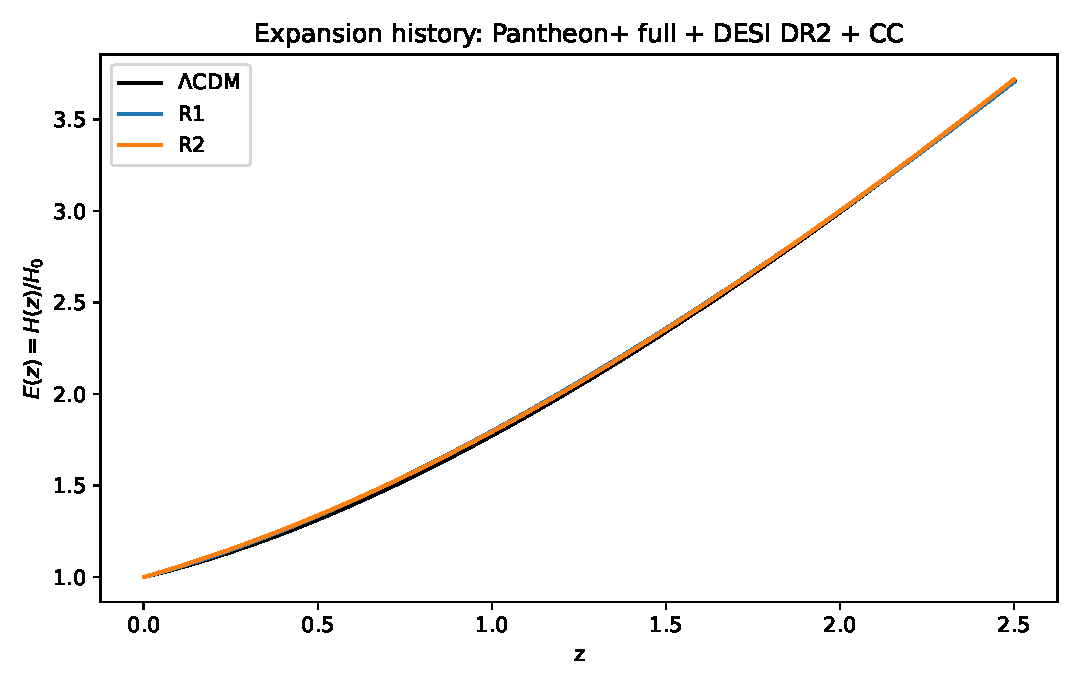
\includegraphics[width=0.86\linewidth]{fig01_expansion_Ez.pdf}
\caption{Expansion history $E(z)=H(z)/H_0$ for the Pantheon+ full covariance + DESI DR2 BAO + cosmic-chronometer best fits. R1 remains close to \LCDM but shifts the preferred matter density and introduces a controlled exponent $\theta$.}
\label{fig:expansion}
\end{figure}

\begin{figure}[H]
\centering
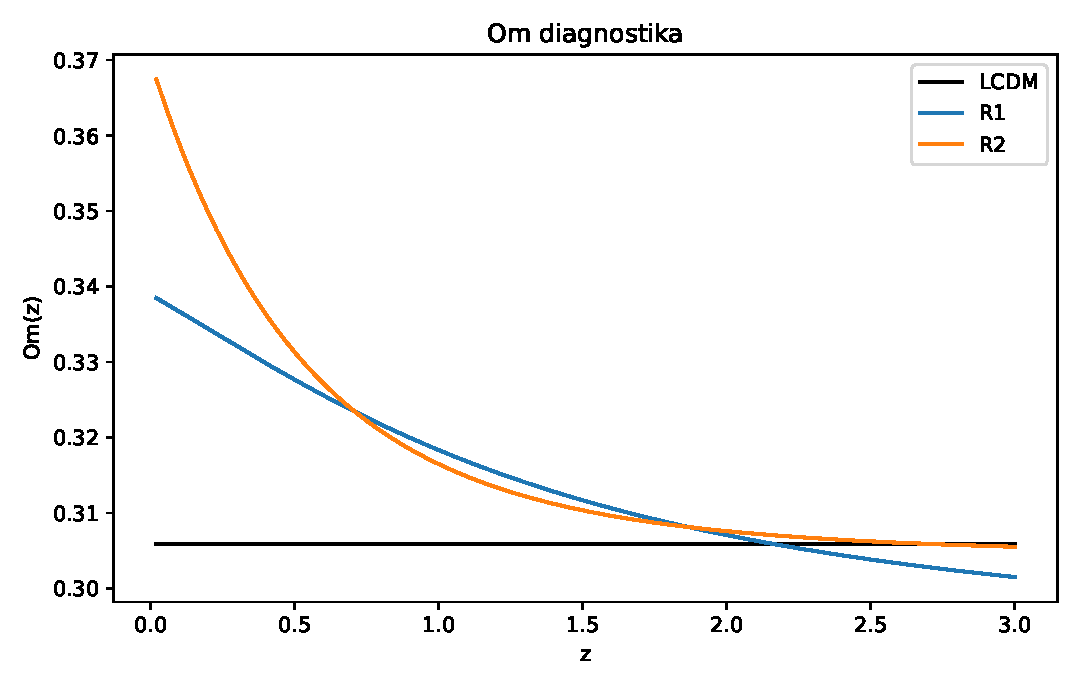
\includegraphics[width=0.86\linewidth]{fig02_om_diagnostic.pdf}
\caption{Om diagnostic. In flat \LCDM, ${\rm Om}(z)$ is constant and equals $\Omega_{\rm m0}$. The R1 and R2 branches predict a redshift drift, providing a direct background-level null test.}
\label{fig:om}
\end{figure}

\begin{figure}[H]
\centering
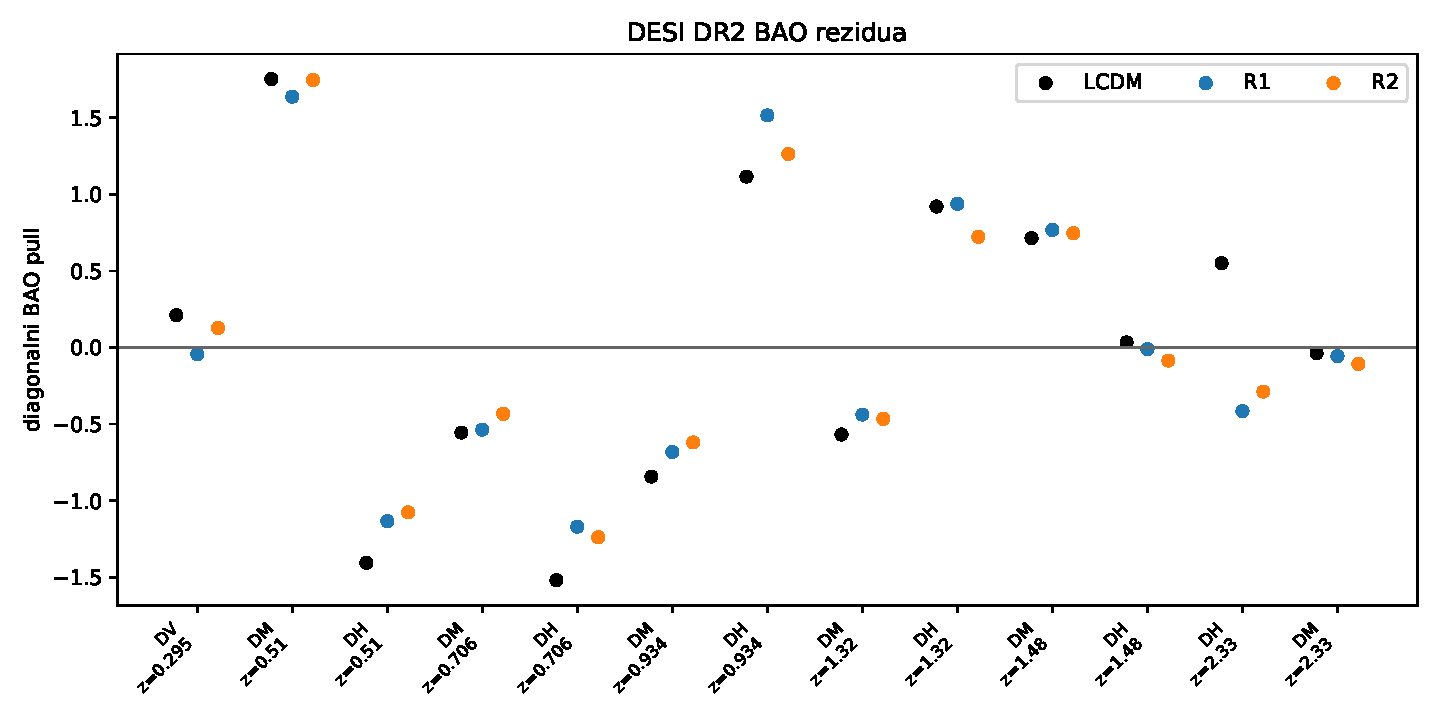
\includegraphics[width=0.98\linewidth]{fig03_desi_dr2_bao_pulls.pdf}
\caption{DESI DR2 BAO diagnostic pulls. The plotted values use diagonal errors only for visual readability; the numerical likelihood uses the full DESI covariance matrix.}
\label{fig:bao}
\end{figure}

\begin{figure}[H]
\centering
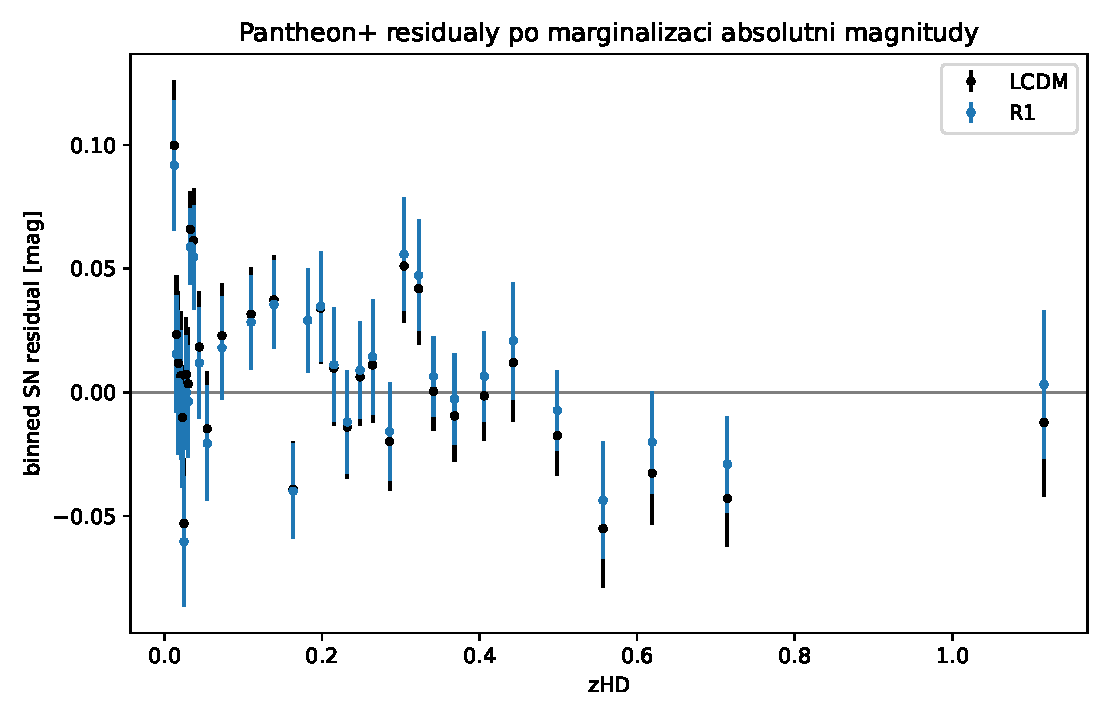
\includegraphics[width=0.86\linewidth]{fig04_pantheon_residuals.pdf}
\caption{Binned Pantheon+ residuals after analytic marginalization over the additive supernova offset. The R1 improvement is distributed over redshift rather than caused by a single outlying point.}
\label{fig:snres}
\end{figure}

\begin{figure}[H]
\centering
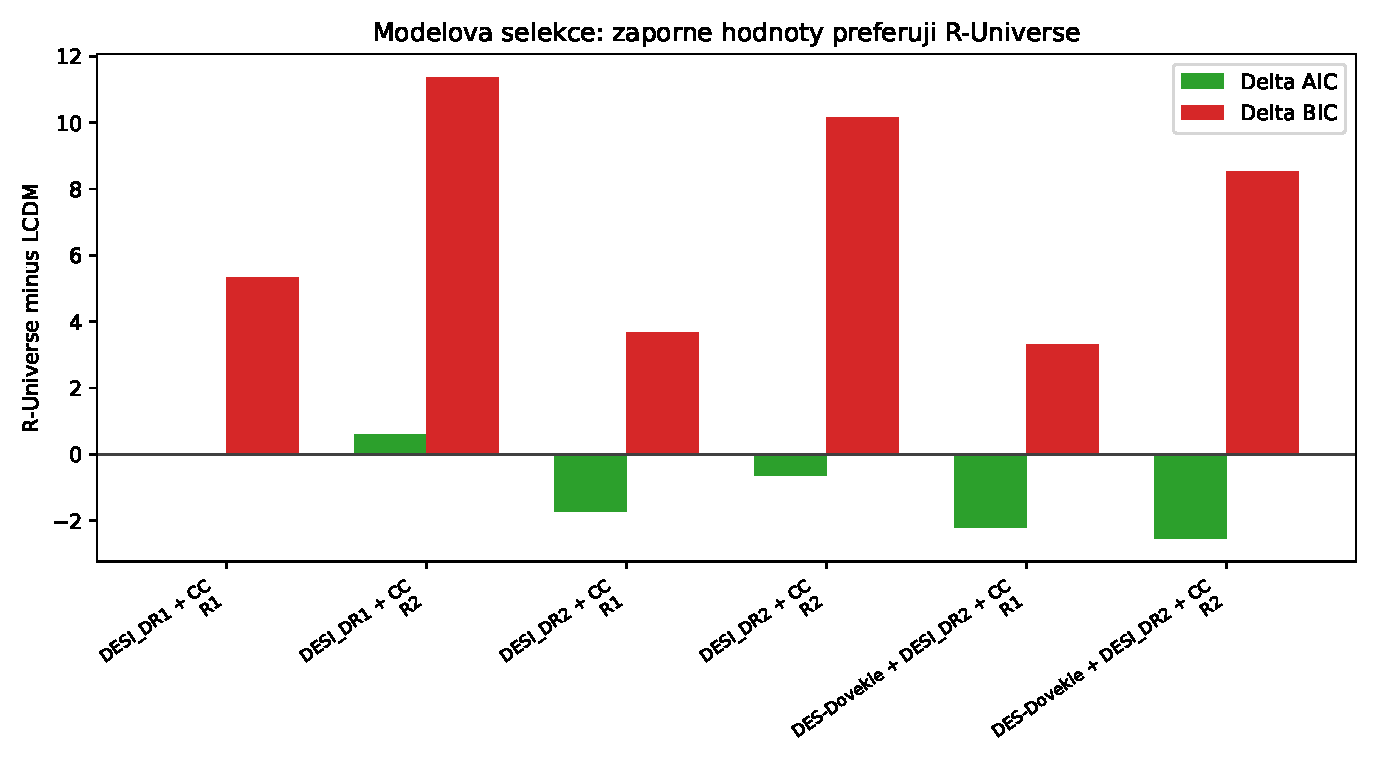
\includegraphics[width=0.96\linewidth]{fig05_model_selection.pdf}
\caption{Information-criterion summary. Negative values favor R-Universe over \LCDM. R1 is AIC-favored in the DESI DR2 and DES-Dovekie configurations but is not BIC-favored.}
\label{fig:modelselection}
\end{figure}

\begin{figure}[H]
\centering
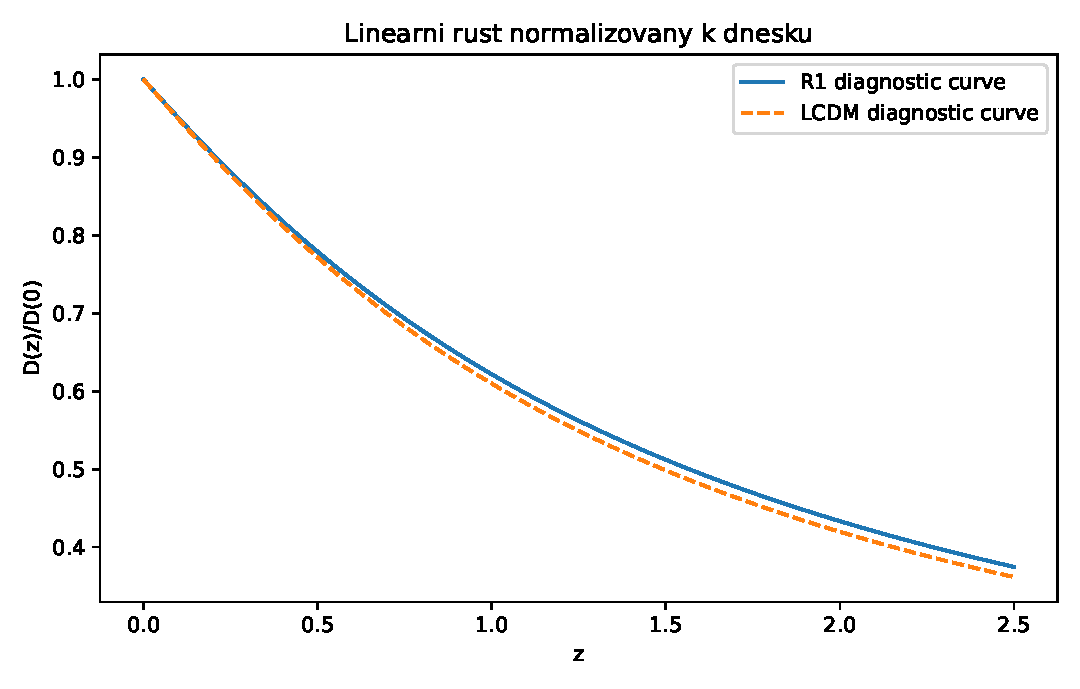
\includegraphics[width=0.82\linewidth]{fig06_growth_Dz.pdf}
\caption{Minimal GR growth solution normalized to $D(0)=1$. This is a closed late-time consistency calculation, not a substitute for a full Boltzmann implementation.}
\label{fig:growth}
\end{figure}


\section{Numerical results}

\subsection{Pantheon+ full covariance + DESI DR1 + chronometers}

\begin{table}[H]
\centering
\caption{Pantheon+ full covariance + DESI DR1 BAO + cosmic chronometers.}
\begin{tabular}{lrrrrrrrr}
\toprule
Model & $k$ & $H_0$ & $\Omega_{\rm m0}$ & $\theta$ & $\nu$ & $\chi^2$ & $\Delta{\rm AIC}$ & $\Delta{\rm BIC}$\\
\midrule
\LCDM & 2 & 68.413 & 0.3116 & 2.000 & 0.000 & 1415.806 & 0 & 0\\
R1 & 3 & 68.050 & 0.2936 & 1.627 & 0.000 & 1413.759 & -0.047 & +5.345\\
R2 & 4 & 68.119 & 0.3169 & 3.727 & 1.314 & 1412.395 & +0.589 & +11.373\\
\bottomrule
\end{tabular}
\end{table}

The full Pantheon+ covariance weakens the earlier diagonal-covariance signal. R1 improves $\chi^2$, but the AIC gain is nearly zero and BIC disfavors it.

\subsection{Pantheon+ full covariance + DESI DR2 + chronometers}

\begin{table}[H]
\centering
\caption{Main fit: Pantheon+ full covariance + DESI DR2 BAO + cosmic chronometers.}
\begin{tabular}{lrrrrrrrr}
\toprule
Model & $k$ & $H_0$ & $\Omega_{\rm m0}$ & $\theta$ & $\nu$ & $\chi^2$ & $\Delta{\rm AIC}$ & $\Delta{\rm BIC}$\\
\midrule
\LCDM & 2 & 68.631 & 0.3059 & 2.000 & 0.000 & 1414.090 & 0 & 0\\
R1 & 3 & 67.975 & 0.2928 & 1.615 & 0.000 & 1410.378 & -1.712 & +3.681\\
R2 & 4 & 67.894 & 0.3045 & 2.408 & 0.508 & 1409.444 & -0.646 & +10.139\\
\bottomrule
\end{tabular}
\end{table}

For R1, the component breakdown is
\begin{align}
\Delta\chi^2_{\rm SN}&=-2.503,\\
\Delta\chi^2_{\rm BAO}&=-1.270,\\
\Delta\chi^2_{\rm CC}&=+0.061.
\end{align}
Thus the signal is shared by supernovae and BAO rather than coming from a single data block.

\subsection{DES-Dovekie + DESI DR2 + chronometers}

\begin{table}[H]
\centering
\caption{Independent supernova cross-check: DES-Dovekie STAT+SYS + DESI DR2 BAO + cosmic chronometers.}
\begin{tabular}{lrrrrrrrr}
\toprule
Model & $k$ & $H_0$ & $\Omega_{\rm m0}$ & $\theta$ & $\nu$ & $\chi^2$ & $\Delta{\rm AIC}$ & $\Delta{\rm BIC}$\\
\midrule
\LCDM & 2 & 68.544 & 0.3076 & 2.000 & 0.000 & 1659.504 & 0 & 0\\
R1 & 3 & 67.944 & 0.2916 & 1.593 & 0.000 & 1655.291 & -2.213 & +3.317\\
R2 & 4 & 67.819 & 0.3131 & 3.244 & 1.074 & 1652.965 & -2.540 & +8.521\\
\bottomrule
\end{tabular}
\end{table}

The DES-Dovekie cross-check reproduces the direction of the R1 signal outside the Pantheon+ pipeline. It remains AIC-favored but not BIC-favored.

\section{Falsifiable predictions}

For the main R1 branch,
\begin{align}
\theta &= 1.61484,\\
q_0 &= -0.49164,\\
j_0 &= 0.93419,\\
w_R(0)&=-0.93473,\\
w_R(1)&=-0.85249,\\
H_\infty/H_0&=0.80695.
\end{align}
The strongest null tests are:
\begin{enumerate}
\item $\theta=2$ must be recovered if future data prefer \LCDM;
\item ${\rm Om}(z)$ must show the predicted R1 drift rather than a constant value;
\item the jerk must deviate from $j_0=1$ at the level implied by the fitted $\theta$;
\item the $fD$ suppression and ISW proxy must survive a full perturbation calculation;
\item a global MCMC or nested-sampling analysis must preserve the AIC gain and ideally cross the BIC threshold.
\end{enumerate}

\section{What is complete and what remains open}

The late-time chain is complete: the physical principle is stated, the background equation is closed, the \LCDM limit is exact, all likelihood observables are computed, the public data sources are named, and the numerical results are generated by code.

The fundamental theory chain is not yet complete. A final replacement of \LCDM requires:
\begin{enumerate}
\item a covariant action or complete field equations for the R-sector;
\item a theoretical calculation of $\theta$ from a specified RG stability matrix;
\item a ghost and gradient-stability analysis;
\item a CLASS/CAMB implementation including radiation, baryons, neutrinos and recombination;
\item a full CMB likelihood;
\item full MCMC or nested-sampling evidence.
\end{enumerate}
These are not optional. They are the next falsification gates.

\section{Conclusion}

R-Universe R1 is a closed, reproducible, one-parameter late-time extension of flat \LCDM. It exactly contains \LCDM at $\theta=2$, computes all late-time distance observables, uses full covariance where available, includes an independent DES-Dovekie supernova cross-check, and gives explicit growth and CMB-proxy predictions under a stated minimal closure.

The empirical result is precise. Pantheon+ full covariance + DESI DR2 + chronometers gives $\Delta\chi^2=-3.7117$ and $\Delta{\rm AIC}=-1.7117$. DES-Dovekie + DESI DR2 + chronometers gives $\Delta\chi^2=-4.2133$ and $\Delta{\rm AIC}=-2.2133$. In both cases BIC remains positive. The model is therefore not yet a definitive replacement for \LCDM, but it is a serious AIC-supported, falsifiable extension whose next required test is a full Boltzmann-level and MCMC analysis.

\bibliographystyle{unsrtnat}
\bibliography{references}

\end{document}
